
% Default to the notebook output style

    


% Inherit from the specified cell style.




    
\documentclass[11pt]{article}

    
    
    \usepackage[T1]{fontenc}
    % Nicer default font (+ math font) than Computer Modern for most use cases
    \usepackage{mathpazo}

    % Basic figure setup, for now with no caption control since it's done
    % automatically by Pandoc (which extracts ![](path) syntax from Markdown).
    \usepackage{graphicx}
    % We will generate all images so they have a width \maxwidth. This means
    % that they will get their normal width if they fit onto the page, but
    % are scaled down if they would overflow the margins.
    \makeatletter
    \def\maxwidth{\ifdim\Gin@nat@width>\linewidth\linewidth
    \else\Gin@nat@width\fi}
    \makeatother
    \let\Oldincludegraphics\includegraphics
    % Set max figure width to be 80% of text width, for now hardcoded.
    \renewcommand{\includegraphics}[1]{\Oldincludegraphics[width=.8\maxwidth]{#1}}
    % Ensure that by default, figures have no caption (until we provide a
    % proper Figure object with a Caption API and a way to capture that
    % in the conversion process - todo).
    \usepackage{caption}
    \DeclareCaptionLabelFormat{nolabel}{}
    \captionsetup{labelformat=nolabel}

    \usepackage{adjustbox} % Used to constrain images to a maximum size 
    \usepackage{xcolor} % Allow colors to be defined
    \usepackage{enumerate} % Needed for markdown enumerations to work
    \usepackage{geometry} % Used to adjust the document margins
    \usepackage{amsmath} % Equations
    \usepackage{amssymb} % Equations
    \usepackage{textcomp} % defines textquotesingle
    % Hack from http://tex.stackexchange.com/a/47451/13684:
    \AtBeginDocument{%
        \def\PYZsq{\textquotesingle}% Upright quotes in Pygmentized code
    }
    \usepackage{upquote} % Upright quotes for verbatim code
    \usepackage{eurosym} % defines \euro
    \usepackage[mathletters]{ucs} % Extended unicode (utf-8) support
    \usepackage[utf8x]{inputenc} % Allow utf-8 characters in the tex document
    \usepackage{fancyvrb} % verbatim replacement that allows latex
    \usepackage{grffile} % extends the file name processing of package graphics 
                         % to support a larger range 
    % The hyperref package gives us a pdf with properly built
    % internal navigation ('pdf bookmarks' for the table of contents,
    % internal cross-reference links, web links for URLs, etc.)
    \usepackage{hyperref}
    \usepackage{longtable} % longtable support required by pandoc >1.10
    \usepackage{booktabs}  % table support for pandoc > 1.12.2
    \usepackage[inline]{enumitem} % IRkernel/repr support (it uses the enumerate* environment)
    \usepackage[normalem]{ulem} % ulem is needed to support strikethroughs (\sout)
                                % normalem makes italics be italics, not underlines
    

    
    
    % Colors for the hyperref package
    \definecolor{urlcolor}{rgb}{0,.145,.698}
    \definecolor{linkcolor}{rgb}{.71,0.21,0.01}
    \definecolor{citecolor}{rgb}{.12,.54,.11}

    % ANSI colors
    \definecolor{ansi-black}{HTML}{3E424D}
    \definecolor{ansi-black-intense}{HTML}{282C36}
    \definecolor{ansi-red}{HTML}{E75C58}
    \definecolor{ansi-red-intense}{HTML}{B22B31}
    \definecolor{ansi-green}{HTML}{00A250}
    \definecolor{ansi-green-intense}{HTML}{007427}
    \definecolor{ansi-yellow}{HTML}{DDB62B}
    \definecolor{ansi-yellow-intense}{HTML}{B27D12}
    \definecolor{ansi-blue}{HTML}{208FFB}
    \definecolor{ansi-blue-intense}{HTML}{0065CA}
    \definecolor{ansi-magenta}{HTML}{D160C4}
    \definecolor{ansi-magenta-intense}{HTML}{A03196}
    \definecolor{ansi-cyan}{HTML}{60C6C8}
    \definecolor{ansi-cyan-intense}{HTML}{258F8F}
    \definecolor{ansi-white}{HTML}{C5C1B4}
    \definecolor{ansi-white-intense}{HTML}{A1A6B2}

    % commands and environments needed by pandoc snippets
    % extracted from the output of `pandoc -s`
    \providecommand{\tightlist}{%
      \setlength{\itemsep}{0pt}\setlength{\parskip}{0pt}}
    \DefineVerbatimEnvironment{Highlighting}{Verbatim}{commandchars=\\\{\}}
    % Add ',fontsize=\small' for more characters per line
    \newenvironment{Shaded}{}{}
    \newcommand{\KeywordTok}[1]{\textcolor[rgb]{0.00,0.44,0.13}{\textbf{{#1}}}}
    \newcommand{\DataTypeTok}[1]{\textcolor[rgb]{0.56,0.13,0.00}{{#1}}}
    \newcommand{\DecValTok}[1]{\textcolor[rgb]{0.25,0.63,0.44}{{#1}}}
    \newcommand{\BaseNTok}[1]{\textcolor[rgb]{0.25,0.63,0.44}{{#1}}}
    \newcommand{\FloatTok}[1]{\textcolor[rgb]{0.25,0.63,0.44}{{#1}}}
    \newcommand{\CharTok}[1]{\textcolor[rgb]{0.25,0.44,0.63}{{#1}}}
    \newcommand{\StringTok}[1]{\textcolor[rgb]{0.25,0.44,0.63}{{#1}}}
    \newcommand{\CommentTok}[1]{\textcolor[rgb]{0.38,0.63,0.69}{\textit{{#1}}}}
    \newcommand{\OtherTok}[1]{\textcolor[rgb]{0.00,0.44,0.13}{{#1}}}
    \newcommand{\AlertTok}[1]{\textcolor[rgb]{1.00,0.00,0.00}{\textbf{{#1}}}}
    \newcommand{\FunctionTok}[1]{\textcolor[rgb]{0.02,0.16,0.49}{{#1}}}
    \newcommand{\RegionMarkerTok}[1]{{#1}}
    \newcommand{\ErrorTok}[1]{\textcolor[rgb]{1.00,0.00,0.00}{\textbf{{#1}}}}
    \newcommand{\NormalTok}[1]{{#1}}
    
    % Additional commands for more recent versions of Pandoc
    \newcommand{\ConstantTok}[1]{\textcolor[rgb]{0.53,0.00,0.00}{{#1}}}
    \newcommand{\SpecialCharTok}[1]{\textcolor[rgb]{0.25,0.44,0.63}{{#1}}}
    \newcommand{\VerbatimStringTok}[1]{\textcolor[rgb]{0.25,0.44,0.63}{{#1}}}
    \newcommand{\SpecialStringTok}[1]{\textcolor[rgb]{0.73,0.40,0.53}{{#1}}}
    \newcommand{\ImportTok}[1]{{#1}}
    \newcommand{\DocumentationTok}[1]{\textcolor[rgb]{0.73,0.13,0.13}{\textit{{#1}}}}
    \newcommand{\AnnotationTok}[1]{\textcolor[rgb]{0.38,0.63,0.69}{\textbf{\textit{{#1}}}}}
    \newcommand{\CommentVarTok}[1]{\textcolor[rgb]{0.38,0.63,0.69}{\textbf{\textit{{#1}}}}}
    \newcommand{\VariableTok}[1]{\textcolor[rgb]{0.10,0.09,0.49}{{#1}}}
    \newcommand{\ControlFlowTok}[1]{\textcolor[rgb]{0.00,0.44,0.13}{\textbf{{#1}}}}
    \newcommand{\OperatorTok}[1]{\textcolor[rgb]{0.40,0.40,0.40}{{#1}}}
    \newcommand{\BuiltInTok}[1]{{#1}}
    \newcommand{\ExtensionTok}[1]{{#1}}
    \newcommand{\PreprocessorTok}[1]{\textcolor[rgb]{0.74,0.48,0.00}{{#1}}}
    \newcommand{\AttributeTok}[1]{\textcolor[rgb]{0.49,0.56,0.16}{{#1}}}
    \newcommand{\InformationTok}[1]{\textcolor[rgb]{0.38,0.63,0.69}{\textbf{\textit{{#1}}}}}
    \newcommand{\WarningTok}[1]{\textcolor[rgb]{0.38,0.63,0.69}{\textbf{\textit{{#1}}}}}
    
    
    % Define a nice break command that doesn't care if a line doesn't already
    % exist.
    \def\br{\hspace*{\fill} \\* }
    % Math Jax compatability definitions
    \def\gt{>}
    \def\lt{<}
    % Document parameters
    \title{report\_descriptive}
    
    
    

    % Pygments definitions
    
\makeatletter
\def\PY@reset{\let\PY@it=\relax \let\PY@bf=\relax%
    \let\PY@ul=\relax \let\PY@tc=\relax%
    \let\PY@bc=\relax \let\PY@ff=\relax}
\def\PY@tok#1{\csname PY@tok@#1\endcsname}
\def\PY@toks#1+{\ifx\relax#1\empty\else%
    \PY@tok{#1}\expandafter\PY@toks\fi}
\def\PY@do#1{\PY@bc{\PY@tc{\PY@ul{%
    \PY@it{\PY@bf{\PY@ff{#1}}}}}}}
\def\PY#1#2{\PY@reset\PY@toks#1+\relax+\PY@do{#2}}

\expandafter\def\csname PY@tok@w\endcsname{\def\PY@tc##1{\textcolor[rgb]{0.73,0.73,0.73}{##1}}}
\expandafter\def\csname PY@tok@c\endcsname{\let\PY@it=\textit\def\PY@tc##1{\textcolor[rgb]{0.25,0.50,0.50}{##1}}}
\expandafter\def\csname PY@tok@cp\endcsname{\def\PY@tc##1{\textcolor[rgb]{0.74,0.48,0.00}{##1}}}
\expandafter\def\csname PY@tok@k\endcsname{\let\PY@bf=\textbf\def\PY@tc##1{\textcolor[rgb]{0.00,0.50,0.00}{##1}}}
\expandafter\def\csname PY@tok@kp\endcsname{\def\PY@tc##1{\textcolor[rgb]{0.00,0.50,0.00}{##1}}}
\expandafter\def\csname PY@tok@kt\endcsname{\def\PY@tc##1{\textcolor[rgb]{0.69,0.00,0.25}{##1}}}
\expandafter\def\csname PY@tok@o\endcsname{\def\PY@tc##1{\textcolor[rgb]{0.40,0.40,0.40}{##1}}}
\expandafter\def\csname PY@tok@ow\endcsname{\let\PY@bf=\textbf\def\PY@tc##1{\textcolor[rgb]{0.67,0.13,1.00}{##1}}}
\expandafter\def\csname PY@tok@nb\endcsname{\def\PY@tc##1{\textcolor[rgb]{0.00,0.50,0.00}{##1}}}
\expandafter\def\csname PY@tok@nf\endcsname{\def\PY@tc##1{\textcolor[rgb]{0.00,0.00,1.00}{##1}}}
\expandafter\def\csname PY@tok@nc\endcsname{\let\PY@bf=\textbf\def\PY@tc##1{\textcolor[rgb]{0.00,0.00,1.00}{##1}}}
\expandafter\def\csname PY@tok@nn\endcsname{\let\PY@bf=\textbf\def\PY@tc##1{\textcolor[rgb]{0.00,0.00,1.00}{##1}}}
\expandafter\def\csname PY@tok@ne\endcsname{\let\PY@bf=\textbf\def\PY@tc##1{\textcolor[rgb]{0.82,0.25,0.23}{##1}}}
\expandafter\def\csname PY@tok@nv\endcsname{\def\PY@tc##1{\textcolor[rgb]{0.10,0.09,0.49}{##1}}}
\expandafter\def\csname PY@tok@no\endcsname{\def\PY@tc##1{\textcolor[rgb]{0.53,0.00,0.00}{##1}}}
\expandafter\def\csname PY@tok@nl\endcsname{\def\PY@tc##1{\textcolor[rgb]{0.63,0.63,0.00}{##1}}}
\expandafter\def\csname PY@tok@ni\endcsname{\let\PY@bf=\textbf\def\PY@tc##1{\textcolor[rgb]{0.60,0.60,0.60}{##1}}}
\expandafter\def\csname PY@tok@na\endcsname{\def\PY@tc##1{\textcolor[rgb]{0.49,0.56,0.16}{##1}}}
\expandafter\def\csname PY@tok@nt\endcsname{\let\PY@bf=\textbf\def\PY@tc##1{\textcolor[rgb]{0.00,0.50,0.00}{##1}}}
\expandafter\def\csname PY@tok@nd\endcsname{\def\PY@tc##1{\textcolor[rgb]{0.67,0.13,1.00}{##1}}}
\expandafter\def\csname PY@tok@s\endcsname{\def\PY@tc##1{\textcolor[rgb]{0.73,0.13,0.13}{##1}}}
\expandafter\def\csname PY@tok@sd\endcsname{\let\PY@it=\textit\def\PY@tc##1{\textcolor[rgb]{0.73,0.13,0.13}{##1}}}
\expandafter\def\csname PY@tok@si\endcsname{\let\PY@bf=\textbf\def\PY@tc##1{\textcolor[rgb]{0.73,0.40,0.53}{##1}}}
\expandafter\def\csname PY@tok@se\endcsname{\let\PY@bf=\textbf\def\PY@tc##1{\textcolor[rgb]{0.73,0.40,0.13}{##1}}}
\expandafter\def\csname PY@tok@sr\endcsname{\def\PY@tc##1{\textcolor[rgb]{0.73,0.40,0.53}{##1}}}
\expandafter\def\csname PY@tok@ss\endcsname{\def\PY@tc##1{\textcolor[rgb]{0.10,0.09,0.49}{##1}}}
\expandafter\def\csname PY@tok@sx\endcsname{\def\PY@tc##1{\textcolor[rgb]{0.00,0.50,0.00}{##1}}}
\expandafter\def\csname PY@tok@m\endcsname{\def\PY@tc##1{\textcolor[rgb]{0.40,0.40,0.40}{##1}}}
\expandafter\def\csname PY@tok@gh\endcsname{\let\PY@bf=\textbf\def\PY@tc##1{\textcolor[rgb]{0.00,0.00,0.50}{##1}}}
\expandafter\def\csname PY@tok@gu\endcsname{\let\PY@bf=\textbf\def\PY@tc##1{\textcolor[rgb]{0.50,0.00,0.50}{##1}}}
\expandafter\def\csname PY@tok@gd\endcsname{\def\PY@tc##1{\textcolor[rgb]{0.63,0.00,0.00}{##1}}}
\expandafter\def\csname PY@tok@gi\endcsname{\def\PY@tc##1{\textcolor[rgb]{0.00,0.63,0.00}{##1}}}
\expandafter\def\csname PY@tok@gr\endcsname{\def\PY@tc##1{\textcolor[rgb]{1.00,0.00,0.00}{##1}}}
\expandafter\def\csname PY@tok@ge\endcsname{\let\PY@it=\textit}
\expandafter\def\csname PY@tok@gs\endcsname{\let\PY@bf=\textbf}
\expandafter\def\csname PY@tok@gp\endcsname{\let\PY@bf=\textbf\def\PY@tc##1{\textcolor[rgb]{0.00,0.00,0.50}{##1}}}
\expandafter\def\csname PY@tok@go\endcsname{\def\PY@tc##1{\textcolor[rgb]{0.53,0.53,0.53}{##1}}}
\expandafter\def\csname PY@tok@gt\endcsname{\def\PY@tc##1{\textcolor[rgb]{0.00,0.27,0.87}{##1}}}
\expandafter\def\csname PY@tok@err\endcsname{\def\PY@bc##1{\setlength{\fboxsep}{0pt}\fcolorbox[rgb]{1.00,0.00,0.00}{1,1,1}{\strut ##1}}}
\expandafter\def\csname PY@tok@kc\endcsname{\let\PY@bf=\textbf\def\PY@tc##1{\textcolor[rgb]{0.00,0.50,0.00}{##1}}}
\expandafter\def\csname PY@tok@kd\endcsname{\let\PY@bf=\textbf\def\PY@tc##1{\textcolor[rgb]{0.00,0.50,0.00}{##1}}}
\expandafter\def\csname PY@tok@kn\endcsname{\let\PY@bf=\textbf\def\PY@tc##1{\textcolor[rgb]{0.00,0.50,0.00}{##1}}}
\expandafter\def\csname PY@tok@kr\endcsname{\let\PY@bf=\textbf\def\PY@tc##1{\textcolor[rgb]{0.00,0.50,0.00}{##1}}}
\expandafter\def\csname PY@tok@bp\endcsname{\def\PY@tc##1{\textcolor[rgb]{0.00,0.50,0.00}{##1}}}
\expandafter\def\csname PY@tok@fm\endcsname{\def\PY@tc##1{\textcolor[rgb]{0.00,0.00,1.00}{##1}}}
\expandafter\def\csname PY@tok@vc\endcsname{\def\PY@tc##1{\textcolor[rgb]{0.10,0.09,0.49}{##1}}}
\expandafter\def\csname PY@tok@vg\endcsname{\def\PY@tc##1{\textcolor[rgb]{0.10,0.09,0.49}{##1}}}
\expandafter\def\csname PY@tok@vi\endcsname{\def\PY@tc##1{\textcolor[rgb]{0.10,0.09,0.49}{##1}}}
\expandafter\def\csname PY@tok@vm\endcsname{\def\PY@tc##1{\textcolor[rgb]{0.10,0.09,0.49}{##1}}}
\expandafter\def\csname PY@tok@sa\endcsname{\def\PY@tc##1{\textcolor[rgb]{0.73,0.13,0.13}{##1}}}
\expandafter\def\csname PY@tok@sb\endcsname{\def\PY@tc##1{\textcolor[rgb]{0.73,0.13,0.13}{##1}}}
\expandafter\def\csname PY@tok@sc\endcsname{\def\PY@tc##1{\textcolor[rgb]{0.73,0.13,0.13}{##1}}}
\expandafter\def\csname PY@tok@dl\endcsname{\def\PY@tc##1{\textcolor[rgb]{0.73,0.13,0.13}{##1}}}
\expandafter\def\csname PY@tok@s2\endcsname{\def\PY@tc##1{\textcolor[rgb]{0.73,0.13,0.13}{##1}}}
\expandafter\def\csname PY@tok@sh\endcsname{\def\PY@tc##1{\textcolor[rgb]{0.73,0.13,0.13}{##1}}}
\expandafter\def\csname PY@tok@s1\endcsname{\def\PY@tc##1{\textcolor[rgb]{0.73,0.13,0.13}{##1}}}
\expandafter\def\csname PY@tok@mb\endcsname{\def\PY@tc##1{\textcolor[rgb]{0.40,0.40,0.40}{##1}}}
\expandafter\def\csname PY@tok@mf\endcsname{\def\PY@tc##1{\textcolor[rgb]{0.40,0.40,0.40}{##1}}}
\expandafter\def\csname PY@tok@mh\endcsname{\def\PY@tc##1{\textcolor[rgb]{0.40,0.40,0.40}{##1}}}
\expandafter\def\csname PY@tok@mi\endcsname{\def\PY@tc##1{\textcolor[rgb]{0.40,0.40,0.40}{##1}}}
\expandafter\def\csname PY@tok@il\endcsname{\def\PY@tc##1{\textcolor[rgb]{0.40,0.40,0.40}{##1}}}
\expandafter\def\csname PY@tok@mo\endcsname{\def\PY@tc##1{\textcolor[rgb]{0.40,0.40,0.40}{##1}}}
\expandafter\def\csname PY@tok@ch\endcsname{\let\PY@it=\textit\def\PY@tc##1{\textcolor[rgb]{0.25,0.50,0.50}{##1}}}
\expandafter\def\csname PY@tok@cm\endcsname{\let\PY@it=\textit\def\PY@tc##1{\textcolor[rgb]{0.25,0.50,0.50}{##1}}}
\expandafter\def\csname PY@tok@cpf\endcsname{\let\PY@it=\textit\def\PY@tc##1{\textcolor[rgb]{0.25,0.50,0.50}{##1}}}
\expandafter\def\csname PY@tok@c1\endcsname{\let\PY@it=\textit\def\PY@tc##1{\textcolor[rgb]{0.25,0.50,0.50}{##1}}}
\expandafter\def\csname PY@tok@cs\endcsname{\let\PY@it=\textit\def\PY@tc##1{\textcolor[rgb]{0.25,0.50,0.50}{##1}}}

\def\PYZbs{\char`\\}
\def\PYZus{\char`\_}
\def\PYZob{\char`\{}
\def\PYZcb{\char`\}}
\def\PYZca{\char`\^}
\def\PYZam{\char`\&}
\def\PYZlt{\char`\<}
\def\PYZgt{\char`\>}
\def\PYZsh{\char`\#}
\def\PYZpc{\char`\%}
\def\PYZdl{\char`\$}
\def\PYZhy{\char`\-}
\def\PYZsq{\char`\'}
\def\PYZdq{\char`\"}
\def\PYZti{\char`\~}
% for compatibility with earlier versions
\def\PYZat{@}
\def\PYZlb{[}
\def\PYZrb{]}
\makeatother


    % Exact colors from NB
    \definecolor{incolor}{rgb}{0.0, 0.0, 0.5}
    \definecolor{outcolor}{rgb}{0.545, 0.0, 0.0}



    
    % Prevent overflowing lines due to hard-to-break entities
    \sloppy 
    % Setup hyperref package
    \hypersetup{
      breaklinks=true,  % so long urls are correctly broken across lines
      colorlinks=true,
      urlcolor=urlcolor,
      linkcolor=linkcolor,
      citecolor=citecolor,
      }
    % Slightly bigger margins than the latex defaults
    
    \geometry{verbose,tmargin=1in,bmargin=1in,lmargin=1in,rmargin=1in}
    
    

    \begin{document}
    
    
    \maketitle
    
    

    
    \section{Отчёт по анализу патентной активности юридических и физических
лиц
России}\label{ux43eux442ux447ux451ux442-ux43fux43e-ux430ux43dux430ux43bux438ux437ux443-ux43fux430ux442ux435ux43dux442ux43dux43eux439-ux430ux43aux442ux438ux432ux43dux43eux441ux442ux438-ux44eux440ux438ux434ux438ux447ux435ux441ux43aux438ux445-ux438-ux444ux438ux437ux438ux447ux435ux441ux43aux438ux445-ux43bux438ux446-ux440ux43eux441ux441ux438ux438}

    \subsection{Summary:}\label{summary}

    \begin{quote}
Для анализа даны \textbf{\(328\)} патентных заявки (Patent
applications), поданных \(625\) \textbf{резидентами России} \textbf{в
иностранные патентные офисы} с период \textbf{с \(1\) января \(2017\)
года по \(31\) декабря \(2017\) года}. - \textbf{Юридически}, данные
включают как патентные заявки физических лиц, ИП (individual, \(113\)
или \(0.18\) правообладателей), так и патентные заявки предприятий
(organizations, \(512\) или \(0.82\) правообладателей).\\
* Цифры учётом совместной подачи заявки несколькими компаниями одного
холдинга.
\end{quote}

\begin{quote}
\begin{itemize}
\tightlist
\item
  \textbf{Географически}, правообладатели патентных заявок распределены
  неравномерно распределены. В Москве (\(148\) или \(0.24\)
  правообладателей, с учётом правообладателей, чьи дочерние предприятия
  зарегистрированы за пределами РФ, но имеют права на патент) и за её
  пределами (\(477\) или \(0.76\) правообладателей)*.\\
  * Подробный анализ в срезе каждого региона возможен при дополнительном
  выделении средств на разметку данных и продолжение анализа.
\end{itemize}
\end{quote}

    ** Распределение правообладателей по типу individual or organisation**:
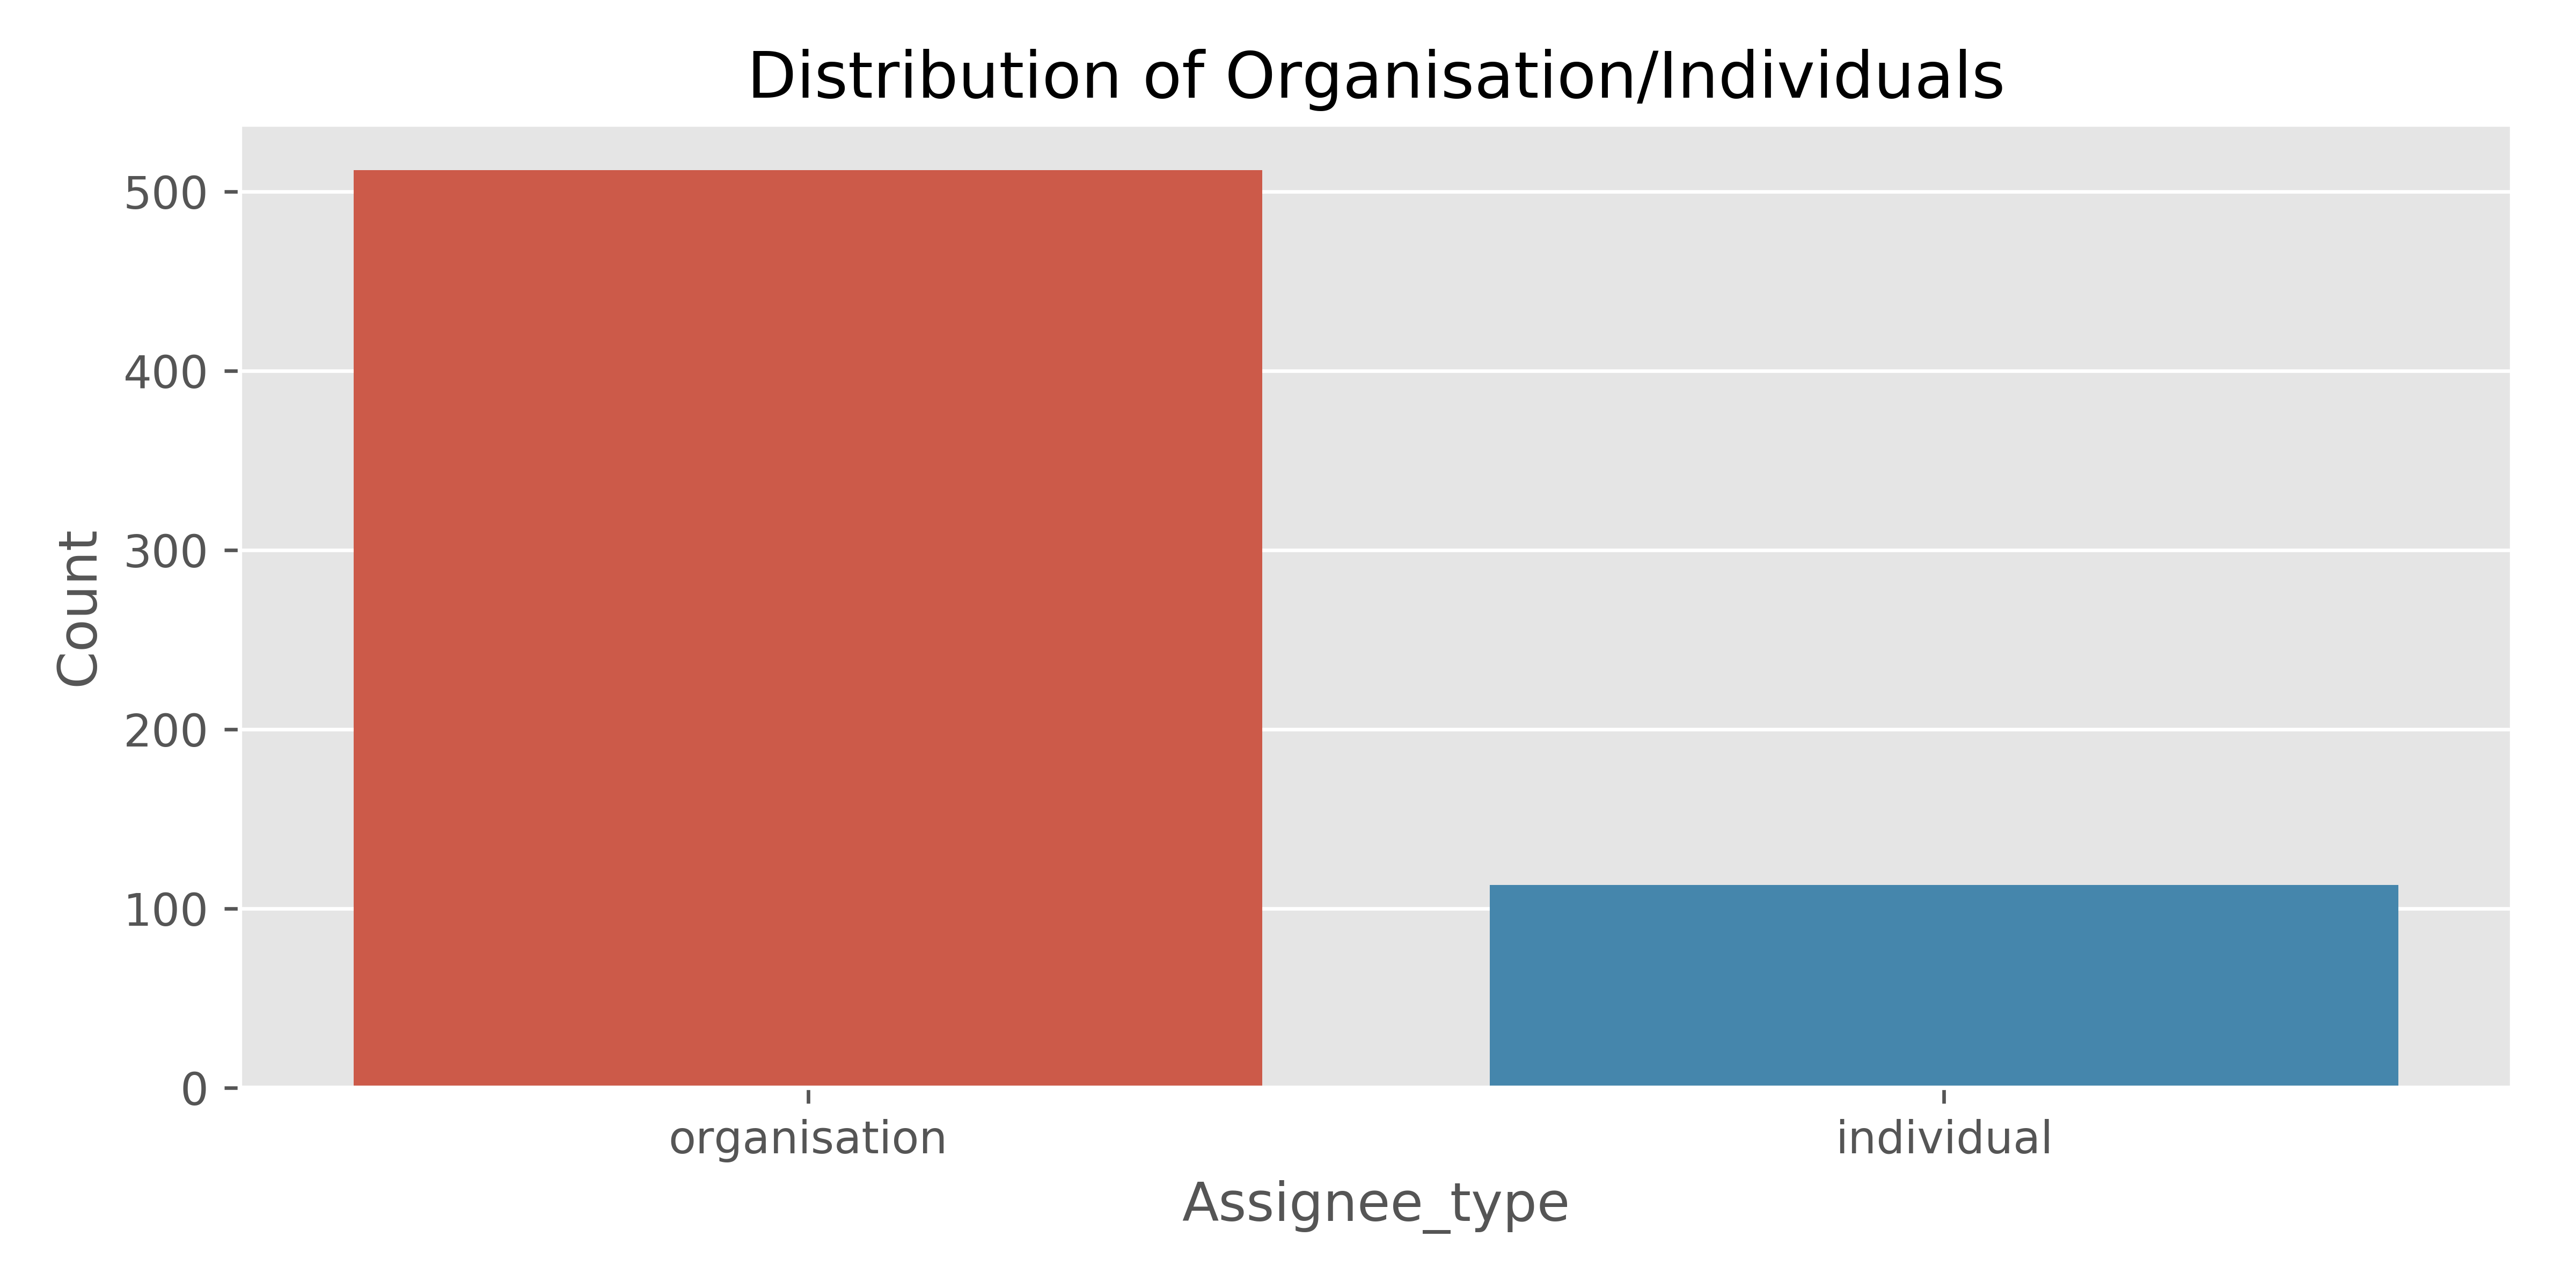
\includegraphics{../reports/figures/Distribution of OrganisationIndividuals.png}

    \textbf{Топ-4 авторы заявок среди организаций (\(0.47\%\) заявок от
организаций)}

\begin{longtable}[]{@{}ll@{}}
\toprule
Автор заявки & Количество заявок\tabularnewline
\midrule
\endhead
Лаборатория Касперского & 121\tabularnewline
INTEL & 50\tabularnewline
Яндекс & 51\tabularnewline
ABBYY & 18\tabularnewline
\bottomrule
\end{longtable}

\textbf{Топ-4 авторы заявок среди individuals (\(0.16\%\) заявок от
individuals)}

\begin{longtable}[]{@{}ll@{}}
\toprule
Автор заявки & Количество заявок\tabularnewline
\midrule
\endhead
ШТОРМ АЛЕКСЕЙ ВИКТОРОВИЧ & 10\tabularnewline
ШИЛОВ ВИКТОР ПЕТРОВИЧ & 4\tabularnewline
УШАКОВ АЛЕКСЕЙ ЛЕОНИДОВИЧ & 2\tabularnewline
ВАРЮХИН МАКСИМ АНТОНОВИЧ & 2\tabularnewline
\bottomrule
\end{longtable}

    \textbf{Алгоритм определения:}\\
распознавание именованных сущностей и ручная обработка сложных случаев.

    ** Распределение правообладателей по региону**:
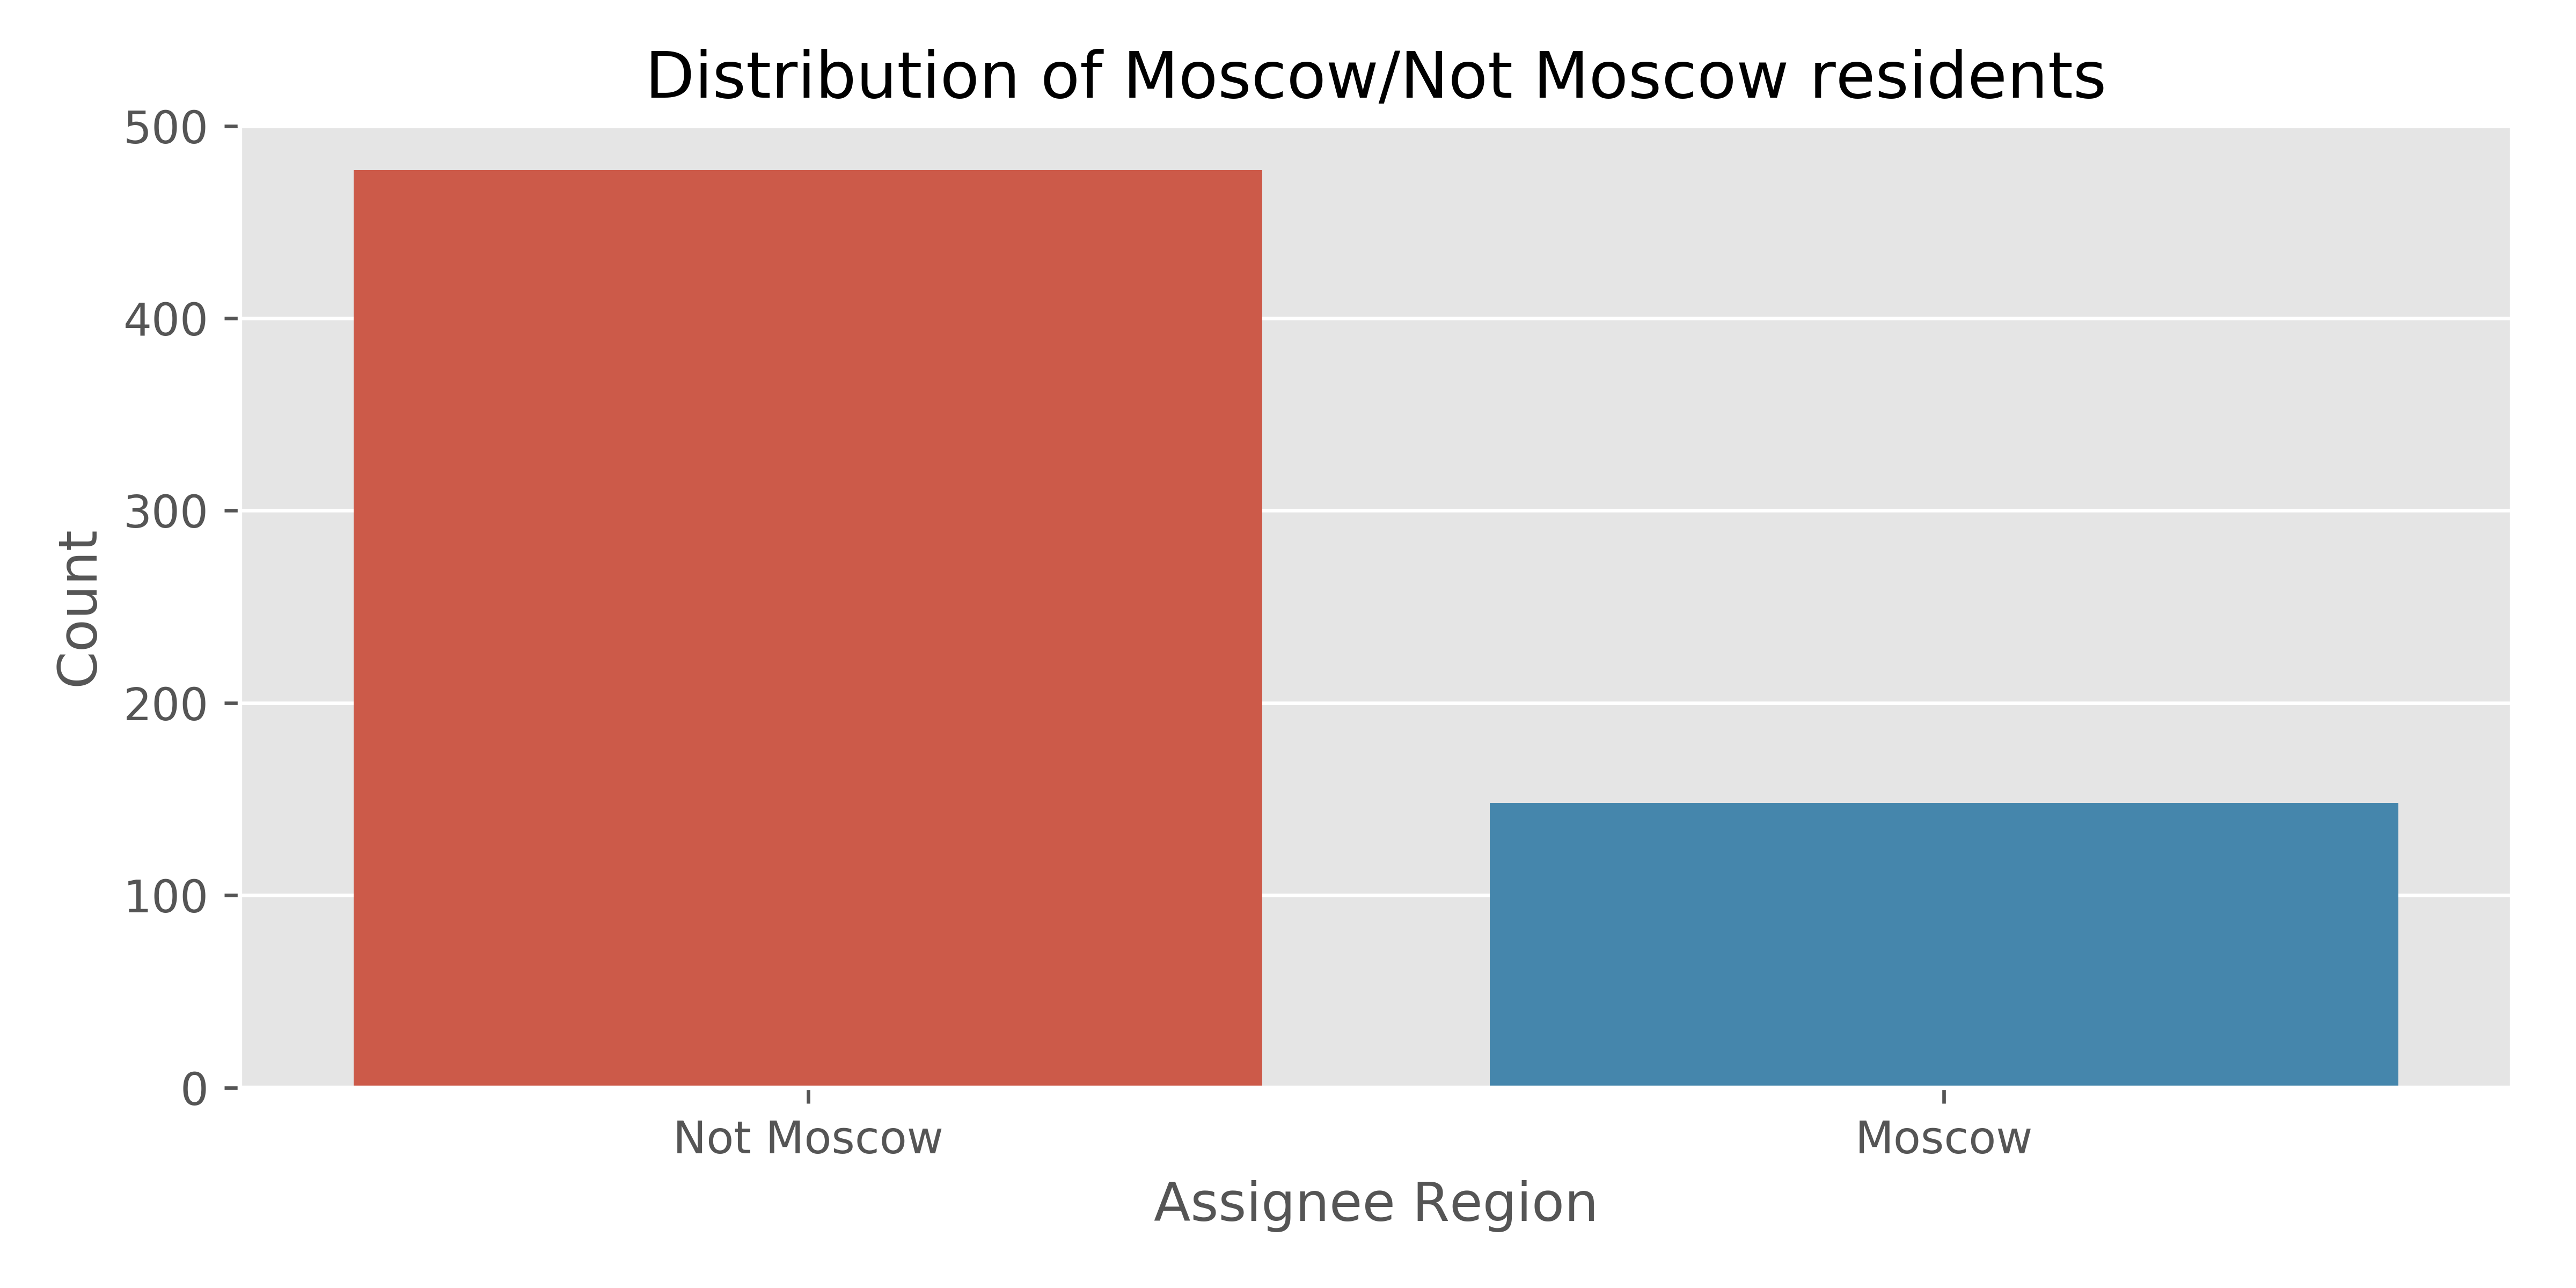
\includegraphics{../reports/figures/Distribution of MoscowNot Moscow residents.png}

    \textbf{Алгоритм обработки:}\\
(переход к следующему пункту если качество работы предыдущего не
устраивает):

\emph{Предобработка:} 0. Перевод транслитного написания в кирилическое

\emph{Поиск:} 0. Ручная обработка крупных Assignees по названиям
холдинга или ФИО. 1. Проверим наличие субъекта Current assignees в
известной базе (Assignee address). 2. Обращение к \emph{открытым}
источникам (в порядке убывания приоритета): * открытые реестры,
налоговые базы, базы проверки контрагентов, базы организаций -
\href{https://egrul.nalog.ru/index.html}{{[}1{]}}
\href{http://zakupki.gov.ru/epz/organization/quicksearch/search.html?searchString=\%D0\%9A\%D0\%B0\%D1\%81\%D0\%BF\%D0\%B5\%D1\%80\%D1\%81\%D0\%BA\%D0\%BE\%D0\%B3\%D0\%BE\&morphology=on\&pageNumber=1\&sortDirection=true\&recordsPerPage=_10\&sortBy=PO_NAZVANIYU\&fz94=on\&fz223=on\&regionDeleted=false}{{[}2{]}}
\href{http://online.igk-group.ru/ru/home?name=\%D0\%90\%D0\%9E+\%22+\%D0\%9B\%D0\%90\%D0\%91\%D0\%9E\%D0\%A0\%D0\%90\%D0\%A2\%D0\%9E\%D0\%A0\%D0\%98\%D0\%AF+\%D0\%9A\%D0\%90\%D0\%A1\%D0\%9F\%D0\%95\%D0\%A0\%D0\%A1\%D0\%9A\%D0\%9E\%D0\%93\%D0\%9E\&ogrn=\&inn=}{{[}3{]}}
\href{https://www.list-org.com/}{{[}4{]}}
\href{https://www.kartoteka.ru/}{{[}5{]}}
\href{https://zachestnyibiznes.ru/}{{[}6{]}}
\href{https://sbis.ru/}{{[}7{]}} \href{https://nalog.io/}{{[}8{]}}, *
базы патентов, базы конкурсов на финансирование -
\href{http://www.findpatent.ru/}{{[}1{]}}
\href{https://patentdb.ru/}{{[}2{]}}
\href{https://4science.ru/}{{[}3{]}}, * обращение к gis сервисам -
\href{https://2gis.ru/}{{[}1{]}}, * ручной поиск.

    \subsection{База PATSTAT}\label{ux431ux430ux437ux430-patstat}

    Так как Orbit не раскрывает свои правила выделения кодов под Technology
domain
\href{https://static.orbit.com/orbit/help/1.9.8/en/index.html\#!Documents/technologydomain.htm}{1},
попробуем выделить их сделав несколько случайных выборок по 1000 с
заданными Technology domain и конкатенировать все уникальные.\\
В качестве запроса к PATSTAT используем
(\href{https://forums.epo.org/coding-with-boolean-operators-for-ipc-codes-5542}{{[}1{]}}
\href{https://forums.epo.org/count-patent-based-on-assignee-country-7832}{{[}2{]}}):

\begin{Shaded}
\begin{Highlighting}[]
\KeywordTok{SELECT} \KeywordTok{DISTINCT}\NormalTok{ a.*}
\KeywordTok{FROM}\NormalTok{ tls201_appln a}
\KeywordTok{JOIN}\NormalTok{ tls209_appln_ipc i }\KeywordTok{ON}\NormalTok{ a.appln_id = i.appln_id}
\KeywordTok{JOIN}\NormalTok{ tls207_pers_appln pa }\KeywordTok{on}\NormalTok{ a.appln_id = pa.appln_id}
\KeywordTok{JOIN}\NormalTok{ tls206_person p }\KeywordTok{on}\NormalTok{ pa.person_id = p.person_id}
\KeywordTok{WHERE}
\NormalTok{(}\KeywordTok{left}\NormalTok{ (ipc_class_symbol, }\DecValTok{4}\NormalTok{) }\KeywordTok{IN}\NormalTok{ (}\StringTok{'H01B'}\NormalTok{, }\StringTok{'F21S'}\NormalTok{, }\StringTok{'C25D'}\NormalTok{, }\StringTok{'H03L'}\NormalTok{, }\StringTok{'H01S'}\NormalTok{, }\StringTok{'H03G'}\NormalTok{, }\StringTok{'F41H'}\NormalTok{, }\StringTok{'H01G'}\NormalTok{, }\StringTok{'G03B'}\NormalTok{, }\StringTok{'E05B'}\NormalTok{, }\StringTok{'B61B'}\NormalTok{, }\StringTok{'B63G'}\NormalTok{, }\StringTok{'H04B'}\NormalTok{, }\StringTok{'G09C'}\NormalTok{, }\StringTok{'B62D'}\NormalTok{, }\StringTok{'B63C'}\NormalTok{, }\StringTok{'H02S'}\NormalTok{, }\StringTok{'F02B'}\NormalTok{, }\StringTok{'H04R'}\NormalTok{, }\StringTok{'G10K'}\NormalTok{, }\StringTok{'G01T'}\NormalTok{, }\StringTok{'G09B'}\NormalTok{, }\StringTok{'G01C'}\NormalTok{, }\StringTok{'G01D'}\NormalTok{, }\StringTok{'F41F'}\NormalTok{, }\StringTok{'A01G'}\NormalTok{, }\StringTok{'H03F'}\NormalTok{, }\StringTok{'E21B'}\NormalTok{, }\StringTok{'F41G'}\NormalTok{, }\StringTok{'B82B'}\NormalTok{, }\StringTok{'G06T'}\NormalTok{, }\StringTok{'C09D'}\NormalTok{, }\StringTok{'H02J'}\NormalTok{, }\StringTok{'G06F'}\NormalTok{, }\StringTok{'C04B'}\NormalTok{, }\StringTok{'G21H'}\NormalTok{, }\StringTok{'B64C'}\NormalTok{, }\StringTok{'H02B'}\NormalTok{, }\StringTok{'E21F'}\NormalTok{, }\StringTok{'H01R'}\NormalTok{, }\StringTok{'H04M'}\NormalTok{, }\StringTok{'B60Q'}\NormalTok{, }\StringTok{'G01F'}\NormalTok{, }\StringTok{'B60V'}\NormalTok{, }\StringTok{'A61L'}\NormalTok{, }\StringTok{'F42C'}\NormalTok{, }\StringTok{'G11C'}\NormalTok{, }\StringTok{'G08G'}\NormalTok{, }\StringTok{'G01N'}\NormalTok{, }\StringTok{'C08J'}\NormalTok{, }\StringTok{'H03H'}\NormalTok{, }\StringTok{'A01K'}\NormalTok{, }\StringTok{'B29C'}\NormalTok{, }\StringTok{'B23K'}\NormalTok{, }\StringTok{'B64G'}\NormalTok{, }\StringTok{'B60R'}\NormalTok{, }\StringTok{'B64F'}\NormalTok{, }\StringTok{'B82Y'}\NormalTok{, }\StringTok{'B66B'}\NormalTok{, }\StringTok{'G06E'}\NormalTok{, }\StringTok{'G08B'}\NormalTok{, }\StringTok{'A61P'}\NormalTok{, }\StringTok{'G05B'}\NormalTok{, }\StringTok{'C08L'}\NormalTok{, }\StringTok{'F25B'}\NormalTok{, }\StringTok{'E03C'}\NormalTok{, }\StringTok{'B62B'}\NormalTok{, }\StringTok{'G02F'}\NormalTok{, }\StringTok{'B23H'}\NormalTok{, }\StringTok{'B22F'}\NormalTok{, }\StringTok{'A61B'}\NormalTok{, }\StringTok{'C23C'}\NormalTok{, }\StringTok{'B44F'}\NormalTok{, }\StringTok{'C07F'}\NormalTok{, }\StringTok{'F21V'}\NormalTok{, }\StringTok{'B64B'}\NormalTok{, }\StringTok{'A47F'}\NormalTok{, }\StringTok{'F16G'}\NormalTok{, }\StringTok{'A61K'}\NormalTok{, }\StringTok{'H04W'}\NormalTok{, }\StringTok{'G01W'}\NormalTok{, }\StringTok{'H01L'}\NormalTok{, }\StringTok{'C12Q'}\NormalTok{, }\StringTok{'H04H'}\NormalTok{, }\StringTok{'G08C'}\NormalTok{, }\StringTok{'C30B'}\NormalTok{, }\StringTok{'B60L'}\NormalTok{, }\StringTok{'B61L'}\NormalTok{, }\StringTok{'F25D'}\NormalTok{, }\StringTok{'G01K'}\NormalTok{, }\StringTok{'G07C'}\NormalTok{, }\StringTok{'H01C'}\NormalTok{, }\StringTok{'E04H'}\NormalTok{, }\StringTok{'G06G'}\NormalTok{, }\StringTok{'H04K'}\NormalTok{, }\StringTok{'C01B'}\NormalTok{, }\StringTok{'G21F'}\NormalTok{, }\StringTok{'H04L'}\NormalTok{, }\StringTok{'G05F'}\NormalTok{, }\StringTok{'G02B'}\NormalTok{, }\StringTok{'B60P'}\NormalTok{, }\StringTok{'G03F'}\NormalTok{, }\StringTok{'C22B'}\NormalTok{, }\StringTok{'F28D'}\NormalTok{, }\StringTok{'B61D'}\NormalTok{, }\StringTok{'C05B'}\NormalTok{, }\StringTok{'H02K'}\NormalTok{, }\StringTok{'G10L'}\NormalTok{, }\StringTok{'H02M'}\NormalTok{, }\StringTok{'F16B'}\NormalTok{, }\StringTok{'G12B'}\NormalTok{, }\StringTok{'F24S'}\NormalTok{, }\StringTok{'B25B'}\NormalTok{, }\StringTok{'G01B'}\NormalTok{, }\StringTok{'B65B'}\NormalTok{, }\StringTok{'G05D'}\NormalTok{, }\StringTok{'C22C'}\NormalTok{, }\StringTok{'C07D'}\NormalTok{, }\StringTok{'C03B'}\NormalTok{, }\StringTok{'G01V'}\NormalTok{, }\StringTok{'H03M'}\NormalTok{, }\StringTok{'G07F'}\NormalTok{, }\StringTok{'H01J'}\NormalTok{, }\StringTok{'G01J'}\NormalTok{, }\StringTok{'H03D'}\NormalTok{, }\StringTok{'A61F'}\NormalTok{, }\StringTok{'H01F'}\NormalTok{, }\StringTok{'G06Q'}\NormalTok{, }\StringTok{'H04Q'}\NormalTok{, }\StringTok{'G06C'}\NormalTok{, }\StringTok{'H03B'}\NormalTok{, }\StringTok{'B65H'}\NormalTok{, }\StringTok{'B23Q'}\NormalTok{, }\StringTok{'E04G'}\NormalTok{, }\StringTok{'G07B'}\NormalTok{, }\StringTok{'B64D'}\NormalTok{, }\StringTok{'G06K'}\NormalTok{, }\StringTok{'G01H'}\NormalTok{, }\StringTok{'F41A'}\NormalTok{, }\StringTok{'C12N'}\NormalTok{, }\StringTok{'F28F'}\NormalTok{, }\StringTok{'B81B'}\NormalTok{, }\StringTok{'H01P'}\NormalTok{, }\StringTok{'H03C'}\NormalTok{, }\StringTok{'E04D'}\NormalTok{, }\StringTok{'A61C'}\NormalTok{, }\StringTok{'G01M'}\NormalTok{, }\StringTok{'B41M'}\NormalTok{, }\StringTok{'H05B'}\NormalTok{, }\StringTok{'G02C'}\NormalTok{, }\StringTok{'F42B'}\NormalTok{, }\StringTok{'H05K'}\NormalTok{, }\StringTok{'H01Q'}\NormalTok{, }\StringTok{'B33Y'}\NormalTok{, }\StringTok{'G09G'}\NormalTok{, }\StringTok{'H04N'}\NormalTok{, }\StringTok{'G11B'}\NormalTok{, }\StringTok{'G01R'}\NormalTok{, }\StringTok{'C01F'}\NormalTok{, }\StringTok{'H03K'}\NormalTok{, }\StringTok{'G01L'}\NormalTok{, }\StringTok{'G09F'}\NormalTok{, }\StringTok{'A45C'}\NormalTok{, }\StringTok{'H04J'}\NormalTok{, }\StringTok{'G01S'}\NormalTok{, }\StringTok{'G06N'}\NormalTok{, }\StringTok{'H02H'}\NormalTok{, }\StringTok{'B42D'}\NormalTok{, }\StringTok{'G07D'}\NormalTok{, }\StringTok{'C09K'}\NormalTok{, }\StringTok{'H02N'}\NormalTok{))}
\KeywordTok{AND}\NormalTok{ appln_filing_year = }\DecValTok{2017}
\KeywordTok{AND}\NormalTok{ appln_auth != }\StringTok{'RU'} \CommentTok{-- Fill to not Russian Office}
\KeywordTok{AND}\NormalTok{ person_ctry_code = }\StringTok{'RU'}  \CommentTok{-- applicant must be from Russia}
\KeywordTok{AND}\NormalTok{ appln_kind = }\StringTok{'A'}  \CommentTok{-- exclude PCT filings where the EPO only served as the Receiving Office}
\KeywordTok{AND}\NormalTok{ a.appln_id < }\DecValTok{900000000}   \CommentTok{-- exclude artificial applications (see PATSTAT Data Catalog for details)}
\end{Highlighting}
\end{Shaded}

\textbf{Cхожесть данных из источников (Orbit, найдено 328 заявок и
PATStAT, найдено 550 заявок):}\\
\emph{Ключ: Колонка} \texttt{Application\ number} \emph{для базы Orbit и
колонка} \texttt{appln\_nr\_original} \emph{для базы PATSTAT:}

Пересекаются \(27\) патентных заяков. Остальные патентные заявки по
заданным полям при заданных условиях не одинаковы. Вероятная проблема в
двух вещах: 1. Неверно сделанный запрос к базе (не все коды technology
domains из базы Orbit найдены). 2. Неверная обработка кодов заявок,
которые в двух базах представлны по разному/с разными названиями.


    % Add a bibliography block to the postdoc
    
    
    
    \end{document}
